\documentclass[12pt,a4paper]{article}

\usepackage[T2A]{fontenc}
\usepackage[utf8]{inputenc}
\usepackage[russian]{babel}

\usepackage{amsmath}
\usepackage{amssymb}
\usepackage{geometry}
\usepackage{graphicx}
\usepackage{hyperref}
\usepackage{indentfirst}
\usepackage{float}
\usepackage{booktabs}
\usepackage{array}

\geometry{
    left=25mm,
    right=25mm,
    top=25mm,
    bottom=25mm
}

\title{
Сравнение алгоритмов скелетизации бинарных изображений:\\
алгоритмы Zhang--Suen и Guo--Hall
}

\author{}
\date{}

\begin{document}

\maketitle

\section{Введение}

Скелетизация бинарных изображений является одной из классических задач цифровой обработки изображений. Ее цель состоит в том, чтобы заменить объект, заданный множеством ненулевых пикселей, более тонким представлением, расположенным приблизительно вдоль центральных линий исходного объекта. Такое представление обычно называют скелетом или медиальной кривой.

В отличие от геометрического подхода Medial Axis Transform, алгоритмы утончения (thinning) работают непосредственно с дискретным изображением. Они последовательно удаляют граничные пиксели объекта, стараясь сохранить связность, концевые точки и общую структуру исходного объекта.

В данной работе рассматриваются два классических алгоритма утончения бинарных изображений:

\begin{itemize}
    \item алгоритм Zhang--Suen 1984 года \cite{zhang1984};
    \item алгоритм Guo--Hall 1989 года \cite{guo1989}.
\end{itemize}

Обе работы относятся к направлению параллельных алгоритмов утончения. В них изображение рассматривается как бинарная матрица, а решение об удалении пикселя принимается на основании локальной окрестности $3\times3$.

Цель работы состоит в том, чтобы разобрать идеи обеих статей, описать математические условия удаления пикселей и сравнить алгоритмы экспериментально по времени работы, числу итераций, размеру итогового скелета и сохранению связности.

\section{Постановка задачи thinning}

Пусть бинарное изображение задано матрицей
\[
    I(i,j) \in \{0,1\}.
\]
Пиксели со значением $1$ образуют объект, а пиксели со значением $0$ образуют фон.

Задача утончения состоит в построении новой бинарной матрицы
\[
    S(i,j) \in \{0,1\},
\]
такой, что множество ненулевых пикселей в $S$ является тонким скелетом исходного объекта.

К алгоритму скелетизации обычно предъявляются следующие требования:

\begin{enumerate}
    \item сохранение связности объекта;
    \item сохранение концевых точек;
    \item уменьшение толщины штрихов до одного пикселя;
    \item расположение результата около центральной линии исходного объекта;
    \item малое число итераций;
    \item простота локальных правил.
\end{enumerate}

В статьях Zhang--Suen и Guo--Hall особое внимание уделяется именно локальности правил и возможности параллельного применения операторов к пикселям изображения \cite{zhang1984,guo1989}.

\section{Окрестность пикселя}

Обе статьи используют окрестность $3\times3$. Центральный пиксель обозначается через $P_1$, а его соседи нумеруются по часовой стрелке:

\[
\begin{array}{ccc}
P_9 & P_2 & P_3 \\
P_8 & P_1 & P_4 \\
P_7 & P_6 & P_5
\end{array}
\]

Значения $P_i$ считаются бинарными:
\[
    P_i \in \{0,1\}.
\]

Такое обозначение удобно, поскольку решение об удалении центрального пикселя $P_1$ формулируется через значения его восьми соседей.

\section{Алгоритм Zhang--Suen}

\subsection{Мотивация статьи}

Статья Zhang и Suen \cite{zhang1984} была направлена на построение быстрого параллельного алгоритма утончения цифровых образов. Авторы рассматривали задачу в контексте распознавания символов, букв, идеографических знаков и других штриховых изображений.

В начале статьи подчеркивается, что в задачах распознавания образов важную роль играет выделение характерных признаков. Для изображений, состоящих из штрихов различной толщины, естественным предварительным шагом является утончение этих штрихов до скелета.

Авторы отмечают, что разные алгоритмы thinning дают разные искажения. Поэтому задача состоит не только в уменьшении толщины штрихов, но и в сохранении формы и связности исходного объекта.

\subsection{Основная идея}

Алгоритм Zhang--Suen состоит из повторяющихся итераций. Каждая итерация делится на две подитерации. В первой подитерации удаляются одни граничные пиксели, во второй - другие.

Такое разбиение важно для сохранения связности. Если удалять все подходящие пиксели полностью параллельно, то возможно разрушение тонких участков объекта. Поэтому авторы используют частичную сериализацию: внутри каждой подитерации пиксели можно обрабатывать параллельно, но две подитерации выполняются последовательно.

\subsection{Число соседей}

Для центрального пикселя $P_1$ вводится величина
\[
    B(P_1)=P_2+P_3+P_4+P_5+P_6+P_7+P_8+P_9.
\]

Она равна числу ненулевых соседей пикселя $P_1$. Условие
\[
    2 \le B(P_1) \le 6
\]
используется для того, чтобы не удалять изолированные точки и концевые пиксели, а также не удалять пиксели, находящиеся глубоко внутри объекта.

\subsection{Число переходов}

Второй важной величиной является $A(P_1)$. Она определяется как число переходов $0\to1$ в циклической последовательности
\[
    P_2, P_3, P_4, P_5, P_6, P_7, P_8, P_9, P_2.
\]

Формально:
\[
\begin{aligned}
A(P_1) ={}&
(1-P_2)P_3 + (1-P_3)P_4 + (1-P_4)P_5 + (1-P_5)P_6 \\
&+ (1-P_6)P_7 + (1-P_7)P_8 + (1-P_8)P_9 + (1-P_9)P_2.
\end{aligned}
\]

Условие
\[
    A(P_1)=1
\]
означает, что единичные соседи центрального пикселя образуют одну связную группу вокруг него. Если удалить такой пиксель, локальная связность объекта с большей вероятностью сохранится.

\subsection{Две подитерации Zhang--Suen}

В первой подитерации пиксель $P_1$ удаляется, если выполнены условия:
\[
    2 \le B(P_1) \le 6,
\]
\[
    A(P_1)=1,
\]
\[
    P_2P_4P_6=0,
\]
\[
    P_4P_6P_8=0.
\]

Во второй подитерации первые два условия сохраняются, но последние два заменяются на:
\[
    P_2P_4P_8=0,
\]
\[
    P_2P_6P_8=0.
\]

Таким образом две подитерации удаляют разные классы граничных и угловых точек. Последовательное применение этих подитераций постепенно сужает объект до скелета.

\subsection{Эксперименты Zhang--Suen}

В статье \cite{zhang1984} авторы демонстрируют работу алгоритма на символе ``H''. В статье показано состояние после первой и второй подитерации, а затем итоговый скелет. Это важно, поскольку позволяет увидеть, что алгоритм не просто применяет абстрактные логические условия, а действительно послойно удаляет граничные пиксели.

Также авторы показывают результаты на разных типах цифровых образов: китайском символе, букве ``B'' и изображении движущегося тела. Удаленные пиксели и пиксели скелета в статье отмечаются разными символами.

Для оценки производительности авторы сравнивают время работы своего алгоритма с более ранними параллельными thinning-алгоритмами Stefanelli--Rosenfeld. Все сравниваемые алгоритмы были реализованы на FORTRAN и запускались на одной машине CDC Cyber 172 \cite{zhang1984}. В статье приведены следующие значения времени работы.

\begin{center}
\begin{tabular}{lccc}
\toprule
Образ & Four-step & Two-step & Zhang--Suen \\
\midrule
Буква B & 0.765 & 0.678 & 0.454 \\
Китайский символ & 1.031 & 0.882 & 0.505 \\
Moving body & 2.713 & 2.221 & 1.163 \\
\bottomrule
\end{tabular}
\end{center}

По этим данным авторы делают вывод, что предложенный алгоритм быстрее сравниваемых методов, при этом визуально получаемые скелеты остаются близкими по качеству \cite{zhang1984}. Отдельно важно, что авторы упоминают экономию памяти: в реализации используются только две матрицы, исходная матрица изображения $IT$ и вспомогательная матрица $M$, в которой отмечаются пиксели, подлежащие удалению.

\section{Алгоритм Guo--Hall}

\subsection{Мотивация статьи}

Работа Guo и Hall \cite{guo1989} появилась через несколько лет после статьи Zhang--Suen. В ней авторы рассматривают более широкий класс двухподитерационных алгоритмов thinning и анализируют их с точки зрения связности, скорости и тонкости результата.

Авторы отмечают, что thinning является фундаментальным предварительным шагом во многих алгоритмах обработки изображений и распознавания образов. Когда объект состоит из штрихов различной толщины, удобно заменить их тонкими медиальными кривыми. Это уменьшает сложность последующей обработки как по времени, так и по памяти.

Главная проблема, обсуждаемая в статье Guo--Hall, состоит в том, что полностью параллельные thinning-алгоритмы с локальной окрестностью $3\times3$ плохо сохраняют связность. Поэтому на практике часто используют частично сериализованные схемы, в которых одна итерация разбивается на несколько подитераций \cite{guo1989}.

\subsection{Цели thinning-алгоритма}

Guo и Hall формулируют несколько целей thinning-алгоритма:

\begin{enumerate}
    \item связность объекта и фона должна сохраняться;
    \item объекты, уже являющиеся кривыми, не должны изменяться;
    \item медиальная кривая должна проходить около середины исходного объекта;
    \item медиальная кривая должна быть как можно более тонкой;
    \item параллельный алгоритм должен требовать как можно меньше итераций.
\end{enumerate}

Эти цели важны, потому что они задают критерии сравнения алгоритмов. В отличие от Zhang--Suen, где основной акцент делается на скорости и простоте, Guo--Hall явно вводят несколько количественных и качественных критериев оценки.

\subsection{Величины $N(P)$ и $C(P)$}

В статье Guo--Hall вводятся дополнительные локальные величины, вычисляемые по окрестности пикселя.

Пусть соседи пикселя $P$ обозначены как $p_1,\ldots,p_8$ по кругу. Тогда вводятся величины
\[
    N_1(P)=
    (p_1\vee p_2)+
    (p_3\vee p_4)+
    (p_5\vee p_6)+
    (p_7\vee p_8),
\]
\[
    N_2(P)=
    (p_2\vee p_3)+
    (p_4\vee p_5)+
    (p_6\vee p_7)+
    (p_8\vee p_1).
\]

После этого определяется
\[
    N(P)=\min(N_1(P),N_2(P)).
\]

Идея такой величины состоит в том, чтобы лучше отличать настоящие концевые точки от лишних пикселей, находящихся в середине толстой кривой.

Также используется величина $C(P)$, которая показывает число связных компонент единиц в восьмисвязной окрестности пикселя. Условие
\[
    C(P)=1
\]
означает, что удаление пикселя не должно разорвать локальную связность объекта.

\subsection{Двухподитерационный алгоритм Guo--Hall}

В одной из схем Guo--Hall пиксель $P$ удаляется, если выполнены условия:
\[
    C(P)=1,
\]
\[
    2 \le N(P) \le 3,
\]
а также одно из дополнительных граничных условий, зависящих от номера подитерации.

В нечетных подитерациях удаляются пиксели, соответствующие одному направлению границы, в четных - противоположному. Таким образом, как и в алгоритме Zhang--Suen, используется частичная сериализация. Однако условия Guo--Hall устроены иначе и направлены на лучшее сохранение связности и получение более тонких медиальных кривых \cite{guo1989}.

\subsection{Идея подполей}

Помимо модификации двухподитерационного алгоритма, Guo и Hall рассматривают второй подход: разбиение изображения на два подполя в шахматном порядке.

Пусть пиксели разбиты на два класса:
\[
    (i+j)\bmod 2 = 0,
\]
\[
    (i+j)\bmod 2 = 1.
\]

На каждой подитерации оператор применяется только к одному из двух подполей. Затем активное подполе меняется. Такой подход также является частичной сериализацией параллельного алгоритма. Его преимущество состоит в том, что за одну подитерацию изменяется только половина пикселей, и это помогает избежать разрушения связности.

\section{Эксперименты Guo--Hall}

Статья Guo--Hall содержит существенно более подробное экспериментальное сравнение, чем работа Zhang--Suen. Авторы сравнивают свои алгоритмы с несколькими двухподитерационными алгоритмами, включая Zhang--Suen, Lii--Wang и Stefanelli--Rosenfeld \cite{guo1989}.

Для сравнения вводятся три метрики:
\[
    m_1
\]
- число итераций до получения медиальной кривой;
\[
    m_2
\]
- процент избыточных пикселей в медиальной кривой;
\[
    m_3
\]
- размер медиальной кривой, то есть число единичных пикселей в результате.

Процент избыточных пикселей определяется как
\[
    m_2 =
    \frac{
    \text{число избыточных пикселей в медиальной кривой}
    }{
    \text{общее число пикселей в медиальной кривой}
    }
    \cdot 100\%.
\]

Под избыточным пикселем понимается пиксель медиальной кривой, который не является концевой точкой, удаление которого не нарушает связность кривой.

\subsection{Трудные тестовые паттерны}

Первый набор экспериментов Guo--Hall построен на специальных трудных паттернах. Среди них линии под углами $135^\circ$ и $45^\circ$, квадрат $2\times2$, квадрат $3\times3$, горизонтальные и вертикальные линии. Эти тесты нужны не для демонстрации красивого результата, а для выявления дефектов алгоритмов.

Например, некоторые алгоритмы могут полностью удалить квадрат $2\times2$ или нарушить связность диагональной линии. Guo и Hall отмечают, что алгоритм Zhang--Suen не всегда сохраняет диагональные линии четной толщины и может не сохранять некоторые малые структуры. Именно поэтому в их работе вводятся более строгие условия удаления пикселей \cite{guo1989}.

\subsection{Наборы естественных и искусственных изображений}

Кроме трудных паттернов, авторы используют четыре набора тестов:

\begin{enumerate}
    \item прямоугольники размера $25\times5$ под углами $0^\circ,15^\circ,\ldots,165^\circ$;
    \item прямоугольники большего размера $40\times8$ с теми же ориентациями;
    \item три английские буквы: A, B и H;
    \item шесть китайских символов.
\end{enumerate}

Такой набор экспериментов важен, потому что он сочетает искусственные и естественные изображения. Искусственные изображения позволяют контролировать геометрию, толщину и ориентацию штрихов, а буквы и китайские символы демонстрируют поведение алгоритма на более реалистичных структурах.

\section{Сравнение Zhang--Suen и Guo--Hall}

Основные различия алгоритмов можно представить следующим образом.

\begin{center}
\begin{tabular}{p{45mm}p{45mm}p{45mm}}
\toprule
Критерий & Zhang--Suen & Guo--Hall \\
\midrule
Год & 1984 & 1989 \\
Основная цель & Быстрый простой параллельный thinning & Улучшение связности, тонкости и скорости \\
Окрестность & $3\times3$ & $3\times3$ \\
Структура итерации & Две подитерации & Две подитерации или два подполя \\
Главные величины & $A(P_1)$, $B(P_1)$ & $C(P)$, $N(P)$ \\
Эксперименты & Символы, буква B, moving body, CPU-время & Трудные паттерны, линии разных ориентаций, буквы, китайские символы, метрики $m_1,m_2,m_3$ \\
Сильная сторона & Простота и скорость & Лучшее сохранение связности и более тонкие результаты \\
\bottomrule
\end{tabular}
\end{center}

Алгоритм Zhang--Suen проще для реализации и хорошо подходит как базовый метод. Его условия удаления пикселей легко записываются и эффективно вычисляются.

Алгоритм Guo--Hall является более детальным развитием той же идеи. Он использует более аккуратные локальные признаки, в частности $C(P)$ и $N(P)$, что позволяет лучше контролировать сохранение связности и концевых точек.

\section{Собственные эксперименты}

\subsection{Постановка эксперимента}

В практической части были реализованы оба алгоритма на C++. Входные изображения хранились в формате PGM. Для каждого изображения программа запускала оба алгоритма и сохраняла два результата: скелет, полученный алгоритмом Zhang--Suen, и скелет, полученный алгоритмом Guo--Hall.

Для каждого запуска измерялись следующие величины:

\begin{itemize}
    \item $P_0$ - число пикселей исходного объекта;
    \item $P$ - число пикселей итогового скелета;
    \item $I$ - число итераций до стабилизации;
    \item $T$ - время работы алгоритма в миллисекундах;
    \item $C_0$ - число восьмисвязных компонент до скелетизации;
    \item $C_1$ - число восьмисвязных компонент после скелетизации.
\end{itemize}

Связность считалась сохраненной, если
\[
    C_0 = C_1.
\]

Важно отметить, что время работы зависит от конкретной машины, компилятора и режима оптимизации. Поэтому в данном эксперименте время используется как практическая характеристика реализации, а число итераций и размер скелета являются более устойчивыми алгоритмическими показателями.

\subsection{Тестовые изображения}

Для эксперимента были использованы следующие изображения:

\begin{itemize}
    \item диагональная линия под углом $45^\circ$;
    \item крест;
    \item ветвящаяся фигура;
    \item гантелеобразная фигура;
    \item зашумленная область;
    \item буквы A, B и H.
\end{itemize}

Такой набор близок к идеологии экспериментов из статей: линии разных ориентаций позволяют проверить поведение алгоритмов на простых геометрических структурах, а буквы и ветвящиеся объекты показывают работу алгоритмов на более сложных штриховых формах.

\subsection{Численные результаты}

Результаты эксперимента приведены в таблице \ref{tab:own_results}. Во всех приведенных тестах оба алгоритма сохранили число восьмисвязных компонент, то есть по выбранной метрике связность объекта не была нарушена.

\begin{table}[H]
\centering
\small
\begin{tabular}{lrrrrrrr}
\toprule
Изображение & $P_0$ & $P_{ZS}$ & $P_{GH}$ & $I_{ZS}$ & $I_{GH}$ & $T_{ZS}$, мс & $T_{GH}$, мс \\
\midrule
Линия $45^\circ$ & 5490 & 154 & 170 & 9 & 17 & 6.89 & 10.21 \\
Крест & 7075 & 257 & 154 & 14 & 78 & 14.11 & 28.78 \\
Ветвление & 5485 & 289 & 257 & 15 & 26 & 9.20 & 10.74 \\
Гантель & 15696 & 86 & 269 & 37 & 95 & 25.48 & 39.95 \\
Зашумленная область & 13085 & 315 & 264 & 47 & 77 & 35.97 & 31.45 \\
Буква A & 9067 & 375 & 453 & 13 & 57 & 9.27 & 23.82 \\
Буква B & 18710 & 422 & 438 & 33 & 71 & 22.79 & 34.36 \\
Буква H & 11803 & 377 & 531 & 16 & 79 & 13.69 & 33.08 \\
\bottomrule
\end{tabular}
\caption{Сравнение результатов Zhang--Suen и Guo--Hall на тестовых изображениях. Здесь $P_0$ - число пикселей исходного объекта, $P_{ZS}$ и $P_{GH}$ - число пикселей скелета, $I_{ZS}$ и $I_{GH}$ - число итераций, $T_{ZS}$ и $T_{GH}$ - время работы.}
\label{tab:own_results}
\end{table}

\subsection{Анализ результатов}

В проведенных запусках Zhang--Suen в среднем требовал меньше итераций и чаще работал быстрее. Например, для буквы H алгоритм Zhang--Suen завершился за 16 итераций, тогда как Guo--Hall потребовал 79 итераций. Похожая картина наблюдается для буквы A, буквы B, креста и гантелеобразной фигуры.

Однако размер итогового скелета не всегда меньше у одного и того же алгоритма. Для креста, ветвления и зашумленной области Guo--Hall дал меньший скелет, чем Zhang--Suen. Для буквы A, буквы B, буквы H, диагональной линии и гантелеобразной фигуры скелет Zhang--Suen оказался меньше.

Этот результат хорошо показывает, что качество thinning-алгоритма нельзя оценивать только по одному числу. Меньшее число пикселей в скелете не всегда означает лучший результат: слишком агрессивное удаление может ухудшить форму или сделать скелет менее похожим на медиальную линию исходного объекта. Поэтому в статьях также рассматриваются связность, число итераций, тонкость медиальной кривой и визуальное качество результата.

\subsection{Визуальное сравнение}

На рисунках \ref{fig:letter_a_compare}--\ref{fig:cross_compare} показаны примеры результатов, полученных двумя алгоритмами. Визуальное сравнение дополняет численные метрики, поскольку скелеты с близким числом пикселей могут иметь разную геометрическую форму.

\begin{figure}[H]
    \centering
    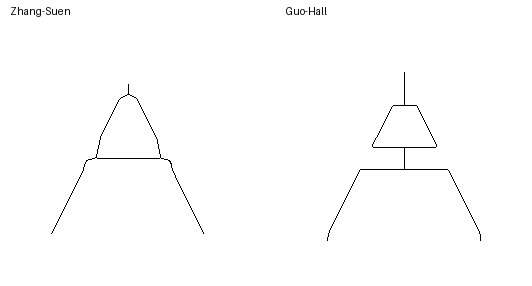
\includegraphics[width=0.85\textwidth]{images/results/letter_a_compare.png}
    \caption{Сравнение результатов для буквы A: слева Zhang--Suen, справа Guo--Hall.}
    \label{fig:letter_a_compare}
\end{figure}

\begin{figure}[H]
    \centering
    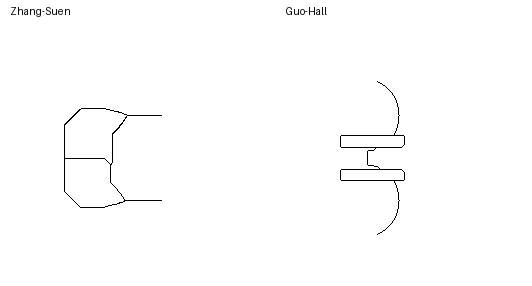
\includegraphics[width=0.85\textwidth]{images/results/letter_b_compare.png}
    \caption{Сравнение результатов для буквы B: слева Zhang--Suen, справа Guo--Hall.}
    \label{fig:letter_b_compare}
\end{figure}

\begin{figure}[H]
    \centering
    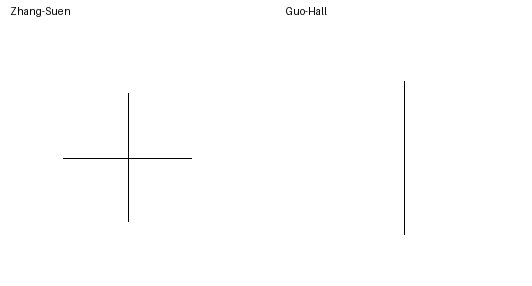
\includegraphics[width=0.85\textwidth]{images/results/cross_compare.png}
    \caption{Сравнение результатов для креста: слева Zhang--Suen, справа Guo--Hall.}
    \label{fig:cross_compare}
\end{figure}

\section{Заключение}

Алгоритмы Zhang--Suen и Guo--Hall являются классическими представителями параллельных алгоритмов thinning с локальной окрестностью $3\times3$.

Работа Zhang--Suen предложила простой и быстрый двухподитерационный алгоритм, хорошо подходящий для распознавания символов и других штриховых изображений \cite{zhang1984}. Работа Guo--Hall развила эту идею и предложила более строгий анализ thinning-алгоритмов с точки зрения связности, тонкости медиальной кривой и параллельной скорости \cite{guo1989}.

Собственные эксперименты показывают, что оба алгоритма сохраняют связность на выбранных тестах, однако различаются по числу итераций, времени работы и размеру полученного скелета. В данной реализации Zhang--Suen чаще оказался быстрее и требовал меньше итераций, тогда как Guo--Hall в некоторых случаях давал более компактный скелет. Это подтверждает общий вывод: сравнение алгоритмов скелетизации должно учитывать не только скорость, но и геометрию результата, сохранение связности и особенности входных изображений.

\begin{thebibliography}{99}

\bibitem{zhang1984}
Zhang T. Y., Suen C. Y.
A Fast Parallel Algorithm for Thinning Digital Patterns //
Communications of the ACM.
1984.
Vol. 27, No. 3.
pp. 236--239.

\bibitem{guo1989}
Guo Z., Hall R. W.
Parallel Thinning with Two-Subiteration Algorithms //
Communications of the ACM.
1989.
Vol. 32, No. 3.
pp. 359--373.

\bibitem{stefanelli1971}
Stefanelli R., Rosenfeld A.
Some Parallel Thinning Algorithms for Digital Pictures //
Journal of the ACM.
1971.
Vol. 18, No. 2.
pp. 255--264.

\bibitem{lam1992}
Lam L., Lee S.-W., Suen C. Y.
Thinning Methodologies -- A Comprehensive Survey //
IEEE Transactions on Pattern Analysis and Machine Intelligence.
1992.
Vol. 14, No. 9.
pp. 869--885.

\end{thebibliography}

\end{document}
